\documentclass{article}
\usepackage{geometry}[margin=0cm]
\usepackage{graphicx}
\usepackage[absolute,overlay]{textpos}

\title{Snake: User Guide}
\author{Alessandra Sasanelli, Simone Maccario}
\date{\today}

\begin{document}
	\maketitle
	\abstract{In this document would like to explain how the game works so a person can easily play. In particular we want to focus on the logic and describe the main keyboard inputs and the initial appstate to run and play it.}
	
	\section{The game}
	
	The goal of the project was to recreate the snake game.\\
	It consists of two basic elements: the snake and the apple and the game's aim is to eat as many apples as possible to increase snake's length.\\
	To make the game more complicate and without having predefined paths, the position of the apple is randomly generated by a function, while the speed of the snake will increase based on how many apples are eaten.\\
	There are two different ways to lose: the first one is when the snake hits itself, the second one is when the snake hits one of the four edges; but no problem, you can play again and again until you get bored.\\
	To interact with the application, it uses simple inputs which are similar to the old inputs used when one of the first snake was released.
	Furthermore, we tried to make the game more fun by using a particular and human sound when the snake eats, while when the player loose, we used a ridiculous game-over.
	
	\section{Command}	
	
	To run the game you just open our game file in Dr.Racket application and run the code and the home page is drawn immediately., 
	Well, now it's time to get to know our commands:\\\\
	\noindent when you are in the home page you can use only
	
	\begin{itemize}
		\item "s" -$>$ using the letter s you can start the game, then the home page disappears and the game draws the game canvas.
	\end{itemize}
	
	\noindent when you are playing the game you can both move the snake or reset the game, notice that the reset button can used also when the game is over
	
	\begin{itemize}
		\item "$\uparrow$" -$>$ using the up arrow you can change the direction of the snake up.
		\item "$\rightarrow$" -$>$ using the right arrow you can change the direction of the snake to the right.
		\item "$\downarrow$" -$>$ using the down arrow you can change the snake's direction to down
		\item "$\leftarrow$" -$>$ using the left arrow you can change the direction of the snake to the left.
		\item "r" -$>$ using the letter r you can restart the game, then the game canvas disappears and the application redraws its home page.
	\end{itemize}
	
	\noindent the last, but not least, command that can be used in every moment, both on the home page and in the game
	
	\begin{itemize}
		\item "esc" -$>$ using the esc button you can exit the game and the game window closes.
	\end{itemize}
	
	\noindent\large{\textbf{IMPORTANT:}}\emph{If you try to change direction in the opposite direction, the snake will not change direction.}\\
	
	\begin{centering}
		\centering Below are three examples of what the canvases look like
	\end{centering}
	
	\begin{textblock*}{10cm}(0cm,9cm)
		\centering
		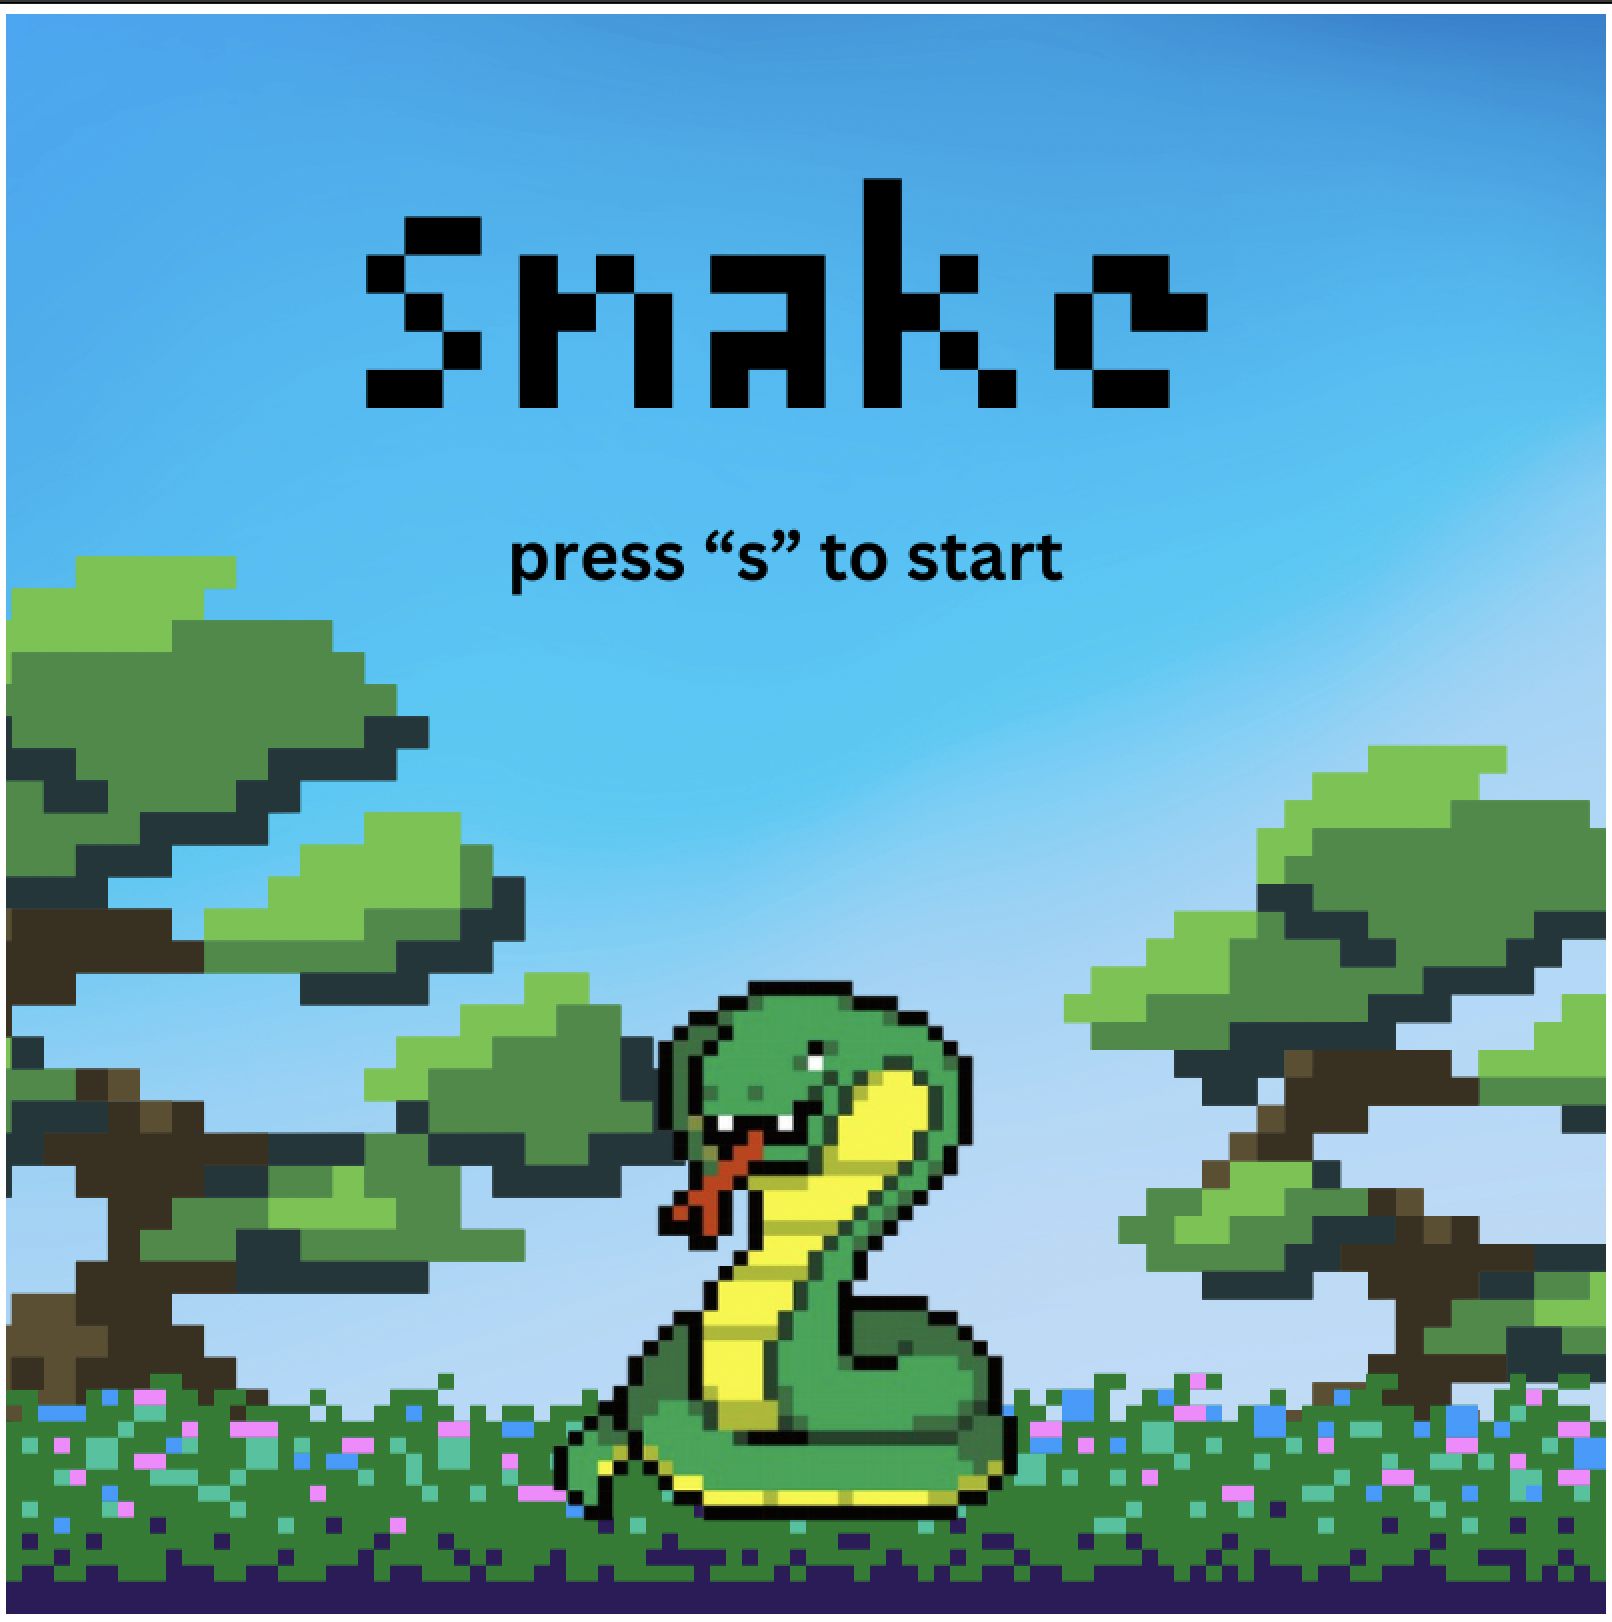
\includegraphics[width=.5\linewidth]{home.png}\\
		\Large{\textbf{Home Page}}
	\end{textblock*}
	
	\begin{textblock*}{10cm}(6cm,9cm)
		\centering
		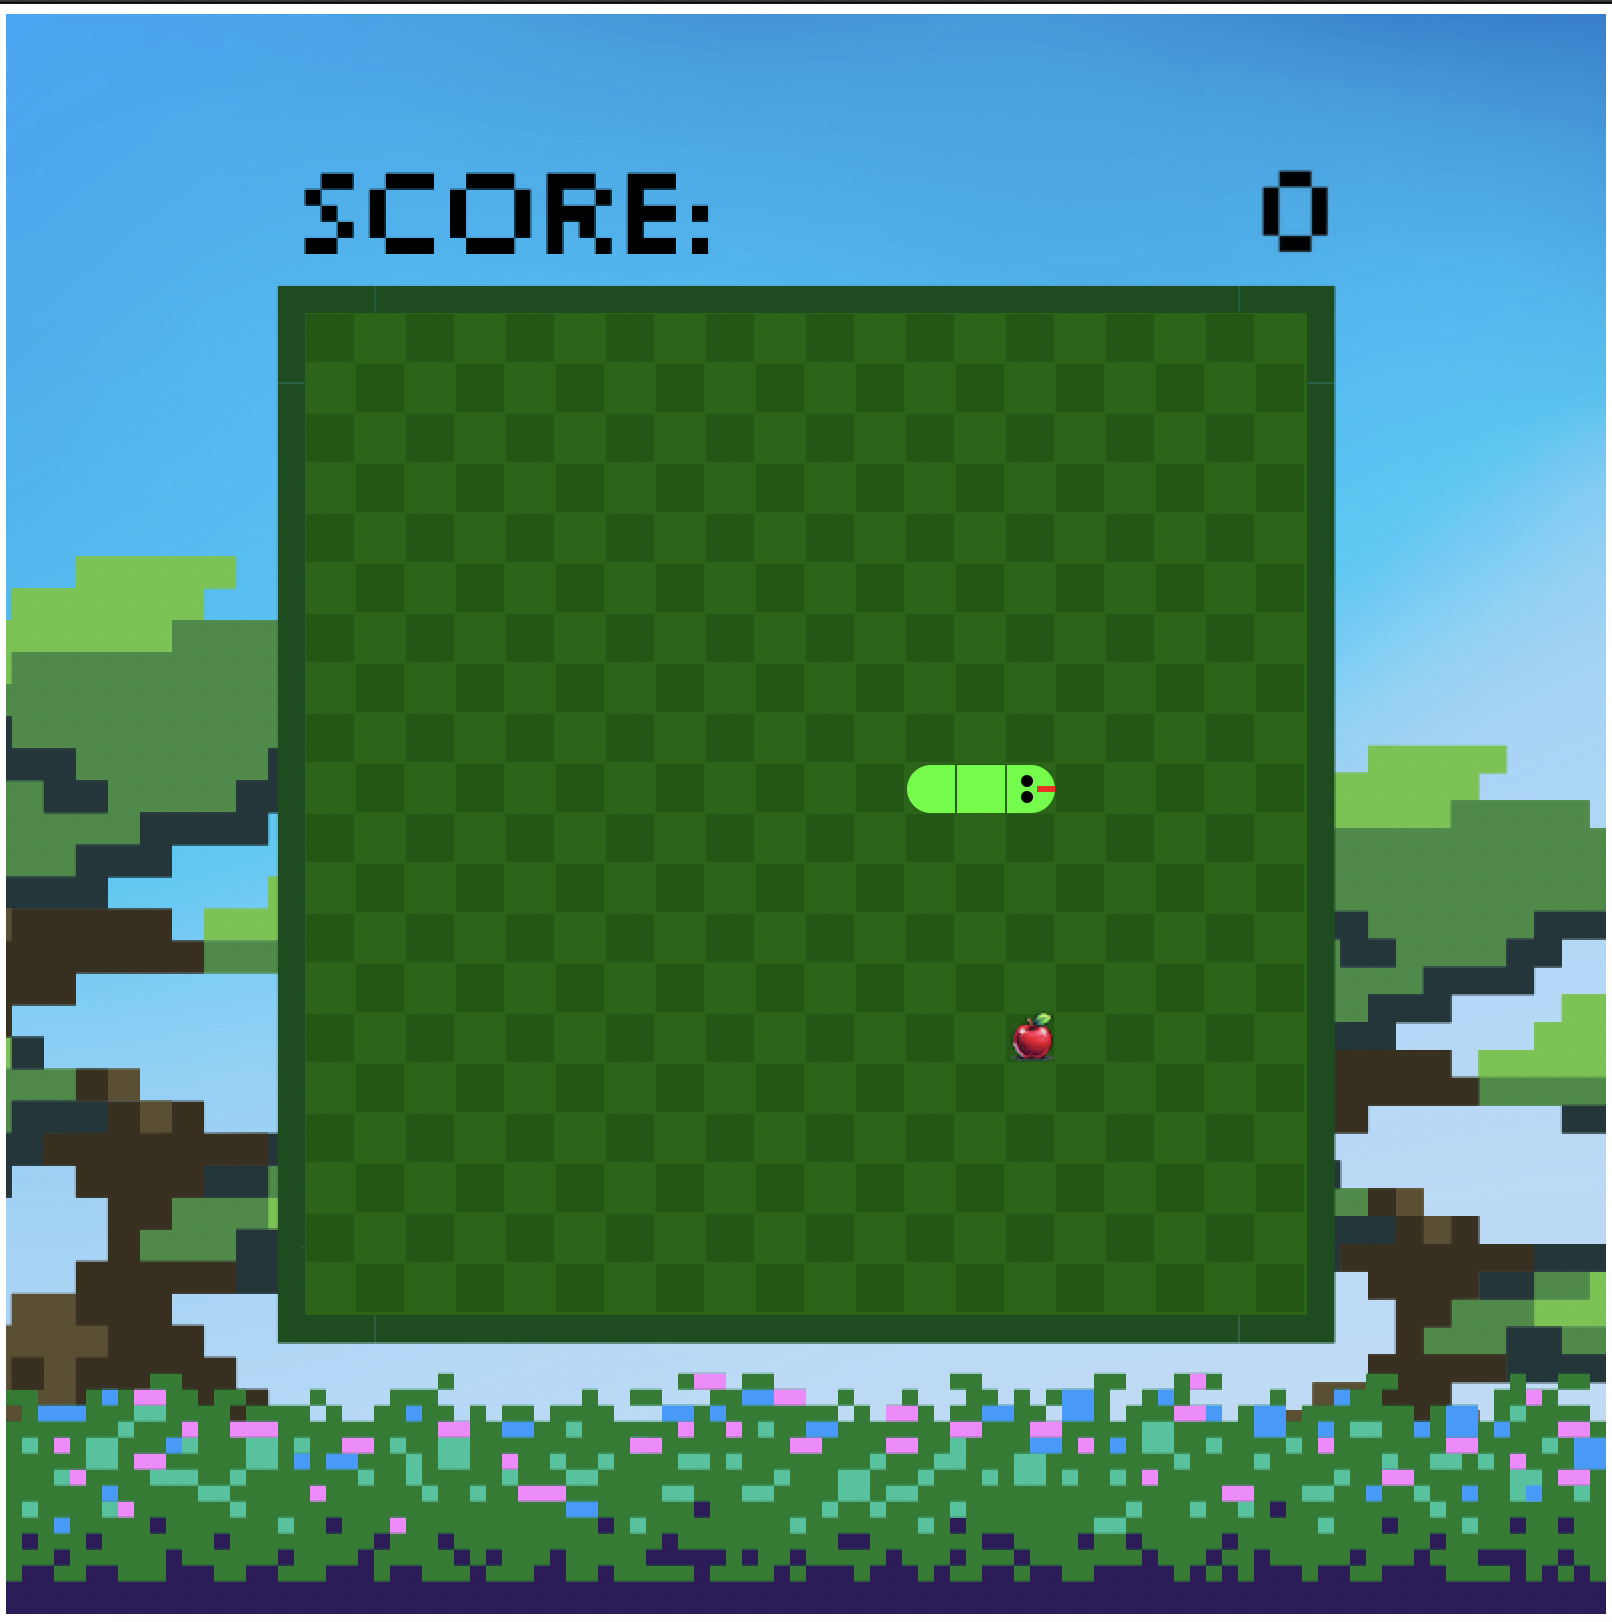
\includegraphics[width=.5\linewidth]{game.png}\\
		\Large{\textbf{Game}}
	\end{textblock*}
	
	\begin{textblock*}{10cm}(12cm,9cm)
		\centering
		
\includegraphics[width=.5\linewidth]{game-over.png}\\
		\Large{\textbf{Game Over}}
	\end{textblock*}
	
	
	
	\vspace{6.5cm}\section{Points}
	As you already know, the aim of the game is to eat the most apple as possible. How the points work and when the snake's speed increases? Well, the score works very simple, at the beginning of every game the number of point is set to 0 by default and every time the snake an apple it scores 100 points and there no limiti except when there is no more space the board.\\
	It's completely different for the speed of the snake, we divided it into eight level in order to start with a low speed to finish with an high one. We also think to give an opportunity to user, In fact, if they want to complicate the game by starting with a higher speed they can. To do this they need only modify a game variable found on line 49 of the "$snake_final.rkt$ "file by setting a positive integer value between 1 and 10, beware: if the value is higher the snake will be too slow	.
	
\end{document}